\documentclass[draft=true,fontsize=12,paper=A4,parskip=half-]{scrbook}
\usepackage[utf8]{inputenc}
\usepackage{ngerman}
\usepackage{pdfpages}
\usepackage{chapterthumb}
\usepackage{xcolor}
\usepackage{tabularx}
\usepackage{titlesec}
\usepackage{nonfloat}
\usepackage{nofloat}
\titleformat{\paragraph}[hang]{\sectfont}{\theparagraph}{.5em}{}
%\usepackage{babel}                                                                                                                  
%\usepackage{ae}                                                                                                                     
%\usepackage{aeguill}                                                                                                                
%\usepackage{shortvrb}                                                                                                               
%\usepackage{tabularx}                                                                                                               
%\usepackage{longtable}                                                                                                              
%\usepackage{amsmath}                                                                                                                
%\usepackage{color}                                                                                                                  
%\usepackage{multirow}                                                                                                               
%\usepackage{ifthen}                                                                                                                 
%\usepackage[DIV12]{typearea}                                                                                                        
%% generated by Docutils <http://docutils.sourceforge.net/>                                                                          
%\setlength{\extrarowheight}{2pt}                                                                                                    
\newlength{\admonitionwidth}                                                                                                        
\setlength{\admonitionwidth}{0.9\textwidth}                                                                                         
\newlength{\docinfowidth}                                                                                                           
\setlength{\docinfowidth}{0.9\textwidth}                                                                                            
\newlength{\locallinewidth}                                                                                                         
\newcommand{\optionlistlabel}[1]{\bf #1 \hfill}                                                                                     
\newenvironment{optionlist}[1]                                                                                                      
{\begin{list}{}                                                                                                                     
  {\setlength{\labelwidth}{#1}                                                                                                      
   \setlength{\rightmargin}{1cm}                                                                                                    
   \setlength{\leftmargin}{\rightmargin}                                                                                            
   \addtolength{\leftmargin}{\labelwidth}                                                                                           
   \addtolength{\leftmargin}{\labelsep}                                                                                             
   \renewcommand{\makelabel}{\optionlistlabel}}                                                                                     
}{\end{list}}                                                                                                                       
\newlength{\lineblockindentation}                                                                                                   
\setlength{\lineblockindentation}{2.5em}                                                                                            
\newenvironment{lineblock}[1]                                                                                                       
{\begin{list}{}                                                                                                                     
  {\setlength{\partopsep}{\parskip}                                                                                                 
   \addtolength{\partopsep}{\baselineskip}                                                                                          
   \topsep0pt\itemsep0.15\baselineskip\parsep0pt                                                                                    
   \leftmargin#1}                                                                                                                   
 \raggedright}                                                                                                                      
{\end{list}}                                                                                                                        
% begin: floats for footnotes tweaking.                                                                                             
\setlength{\floatsep}{0.5em}                                                                                                        
\setlength{\textfloatsep}{\fill}                                                                                                    
\addtolength{\textfloatsep}{3em}                                                                                                    
\renewcommand{\textfraction}{0.5}                                                                                                   
\renewcommand{\topfraction}{0.5}                                                                                                    
\renewcommand{\bottomfraction}{0.5}                                                                                                 
\setcounter{totalnumber}{50}                                                                                                        
\setcounter{topnumber}{50}                                                                                                          
\setcounter{bottomnumber}{50}                                                                                                       
% end floats for footnotes                                                                                                          
% some commands, that could be overwritten in the style file.                                                                       
\newcommand{\rubric}[1]{\subsection*{~\hfill {\it #1} \hfill ~}}                                                                    
\newcommand{\titlereference}[1]{\textsl{#1}}                                                                                        
% end of "some commands"                                                                                                            

\makeglossary
\pagestyle{scrheadings}
\addtokomafont{chapterthumb}{\bfseries}
\selectlanguage{german}
\usepackage[%
    bookmarks=true, 
    bookmarksnumbered=true, 
    bookmarksopen=true, 
    bookmarksopenlevel=1,
    hyperfootnotes=true,
    linktocpage=false,
    colorlinks=true, 
    linkcolor=blue, 
    urlcolor=blue, 
    filecolor=blue,
    linkbordercolor={0 1 1},
    menubordercolor={0 1 1},
    urlbordercolor={1 0 0},
    hyperfootnotes=true,
    hyperindex=true,
    pdfpagelayout=OneColumn, 
    plainpages=false, 
    pdfpagelabels,
    pdftitle={GOsa Komplettdokumentation},
    pdfstartpage={1},
    pdfstartview={FitH}
]{hyperref}


\begin{document}

  \title{GOsa NG}
  \author{Cajus Pollmeier}
  \subtitle{GOsa Komplettdokumentation}
  \publishers{Veröffentlicht vom GOsa-Team}
  \maketitle

  \tableofcontents

  \part{Einführung}

  \ifpdfoutput{\ihead[\putchapterthumb]{\putchapterthumb}}{}
  \chapter{Introduction}


  %\include{installation}
  %\include{configuration}
  \ifpdfoutput{\ihead[]{}}{}

  \part{Benutzerdokumentation}
  \ifpdfoutput{\ihead[\putchapterthumb]{\putchapterthumb}}{}
  %\chapter{Introduction}


  \ifpdfoutput{\ihead[]{}}{}

  \part{Entwicklerdokumentation}
  \ifpdfoutput{\ihead[\putchapterthumb]{\putchapterthumb}}{}
  \chapter{Übersicht}

Dieses Kapitel beschäftigt sich mit den einzelnen GOsa-Komponenten, erklärt
welche Aufgabe sie im Gesamtkonstrukt haben und setzt sie zu einem grossen
Ganzen zusammen. Entwickler-Informationen entnehmen Sie bitte der dem Entwickler
teil dieses Buches.

Die folgenden Unterkapitel beschäftigen sich allesamt mit dieser Grafik:

\begin{minipage}{\linewidth}
 \centering
 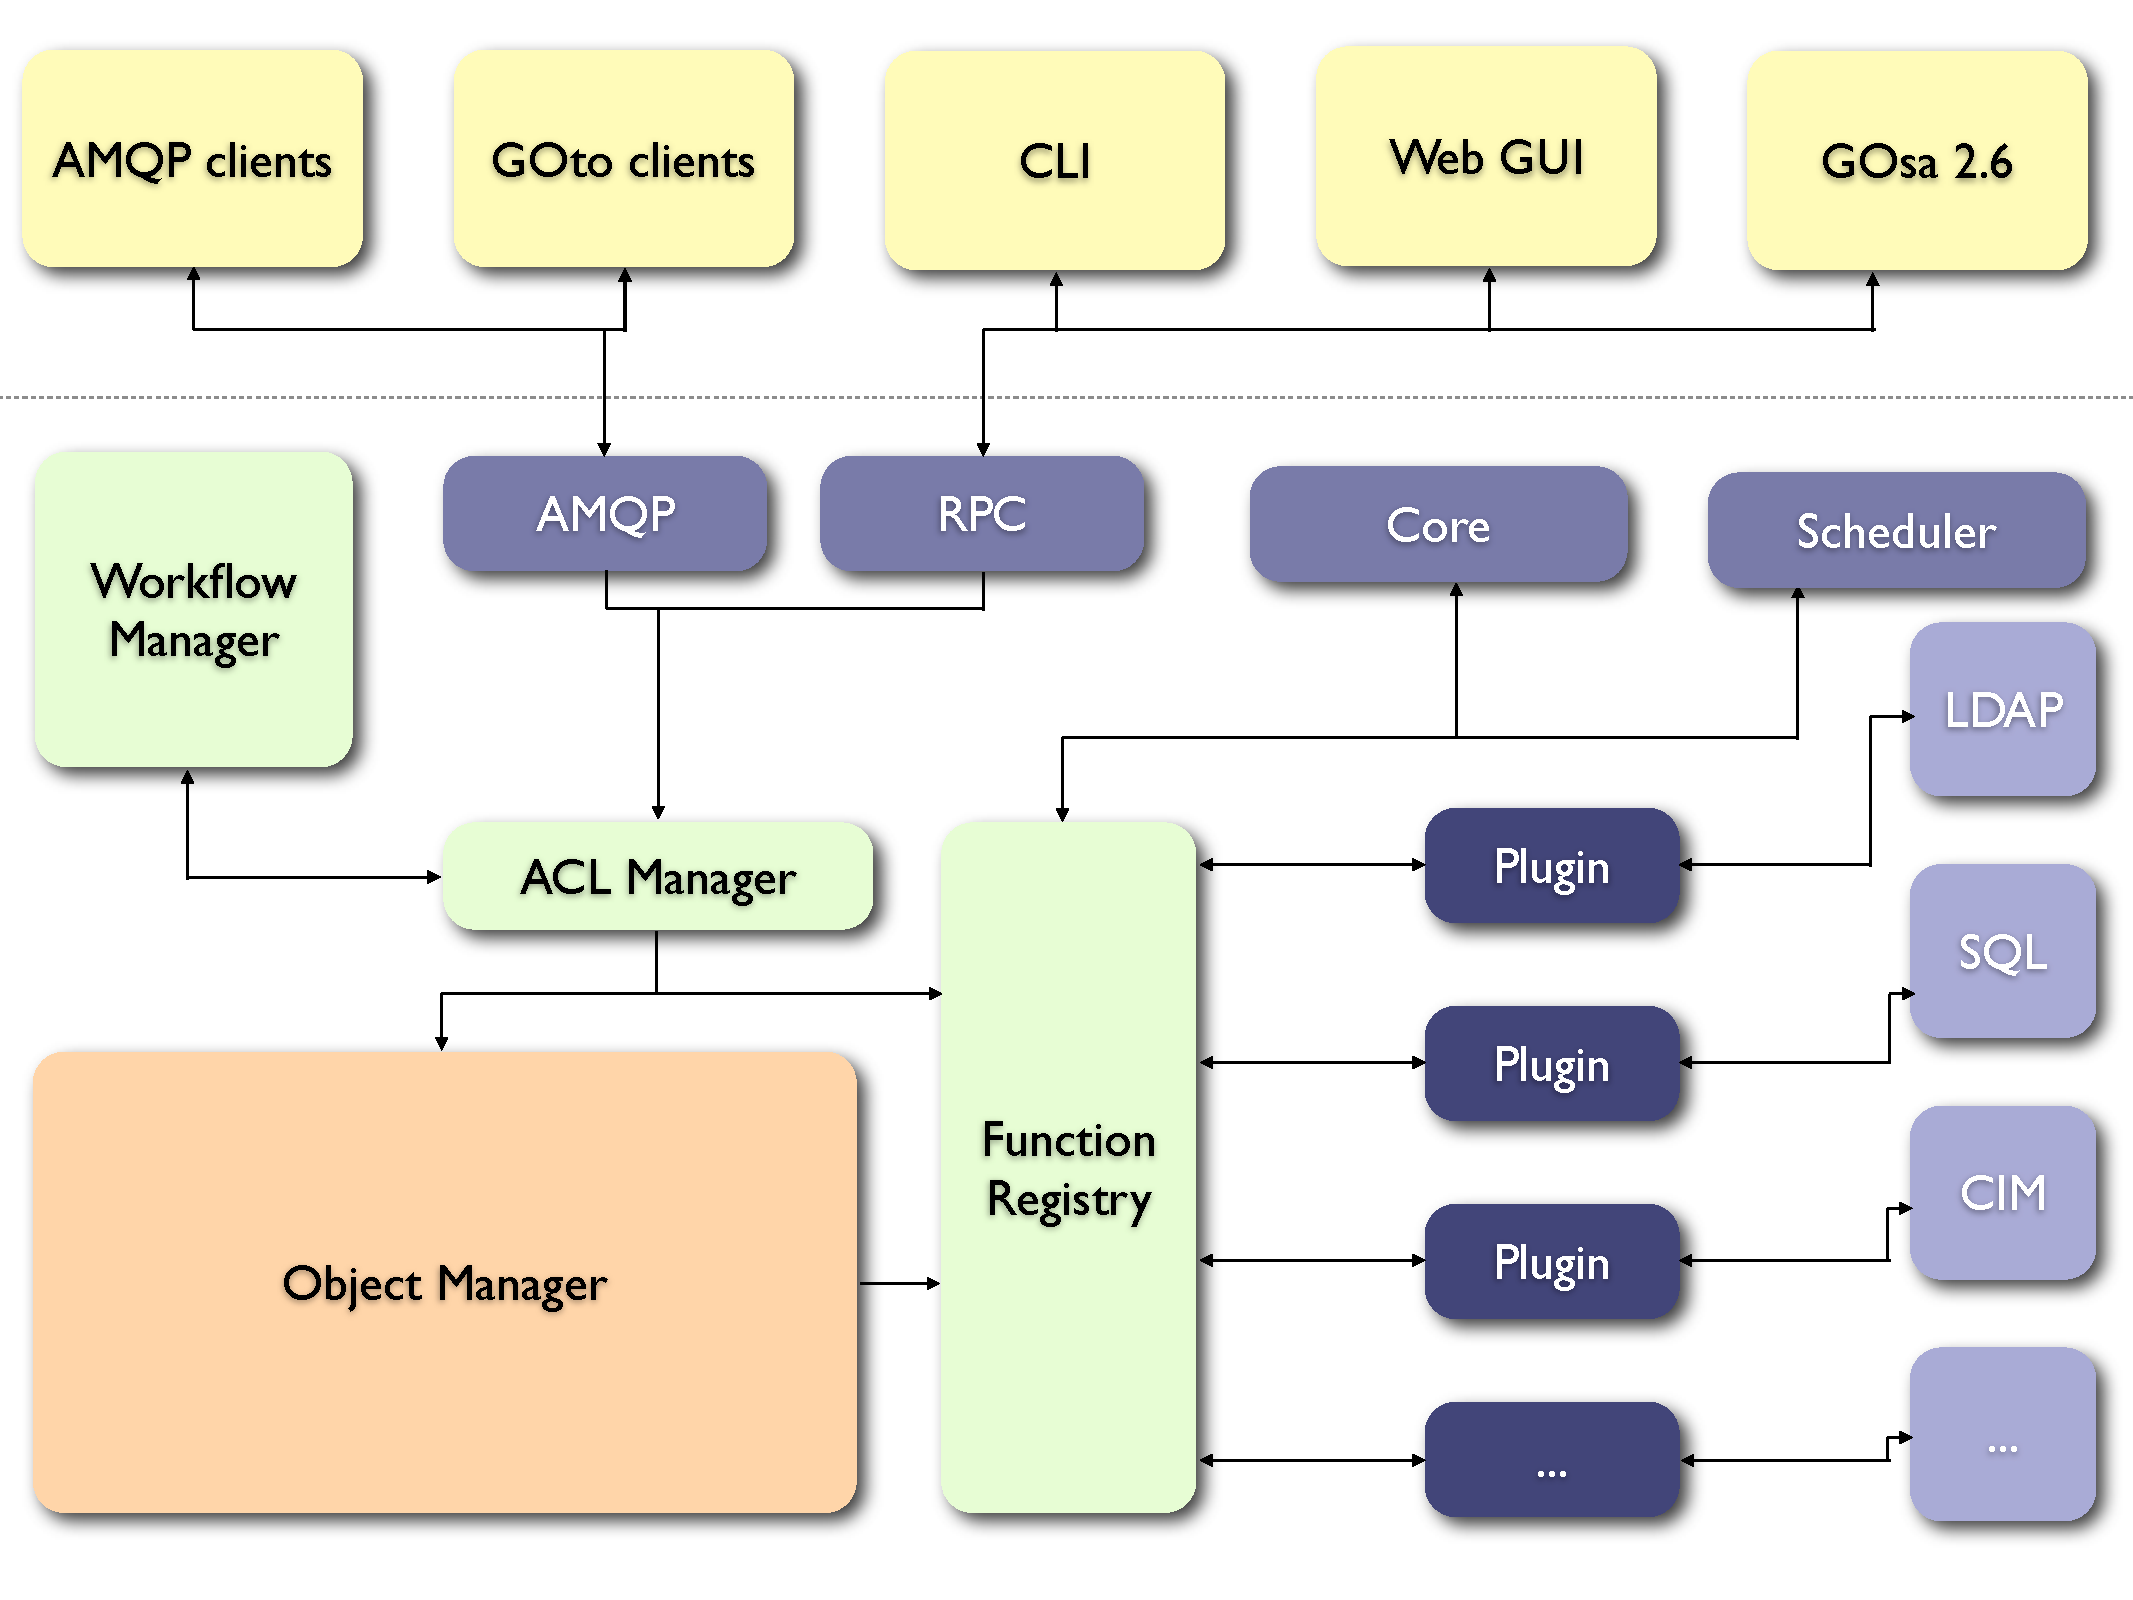
\includegraphics[width=1\textwidth]{media/gosa-design-overview.pdf}
 \figcaption{Komponentenübersicht}
 \label{fig:DesignOverview}
\end{minipage}


\section{Core}

Der GOsa-Kern beinhaltet grundlegende Funktionen, die von allen Modulen
direkt verwendet werden können. Hierbei kann es sich z.B. um das Auflisten
von verfügbaren Objekt-Typen oder die Authentifizierung handeln.

Alle vom Kern bereitgestellten Funktionen werden in der \textit{Function Registry}
registriert und können von dort benutzt werden.


\section{Function Registry}

In der \textit{Function Registry} sind alle aufrufbaren Funktionen hinterlegt.
Plugins, die öffentliche Funktionen bereitstellen müssen sie an dieser Stelle
registrieren. Öffentliche Funktionen lassen sich beispielsweise über einen 
Client über RPC aufrufen.

Ein Überladen von Funktionen ist durch in der Ladenreihenfolge weiter hinten
angeordnete Plugins möglich. Bei Bedarf lassen sich die Funktionen also
überschreiben.

Ausführbar sind diese Funktionen, wenn die Zugriffsrichtlinien das X-Flag 
für diese Funktion vorsehen. Eine Ausführung durch berechtigte Personen
wird damit gewährleistet.


\section{Plugins}

Plugins sind Module die die GOsa-Funktionalität um bestimmte Aspekte erweitern.
So existiert ein Modul für den LDAP- oder Datenbank-Zugriff. Denkbar wäre z.B.
ein Modul das sich um Ihre Zeiterfassung kümmert und die Anwesenheitszeiten
von Benutzern in einer Datenbank pflegt.

Plugins können auf Funktionen der \textit{Function Registry} zurückgreifen und
sind in der Lage GOsa \textit{AMQP-Queues} zu nutzen.

Plugins werden beim Start von GOsa eingebunden.


\section{Scheduler}

Der Scheduler ist das Uhrwerk von GOsa und sorgt dafür das bestimmte Aktionen
zu festgelegten Zeitpunkten - oder gar wiederkehrend - ausgeführt werden.

Module könne sich hier registrieren und werden nach dem gewünschten Zeitplan
benachrichtigt. Die verwendeten Zeitstempel liegen alle in der Zeitzone Z.

\begin{verbatim}
When: once -> timestamp
      loop -> start timestamp
              stop  timestamp
              minute         syntax like cron
              hour
              day_of_month
              month
              day_of_week

What: Job
\end{verbatim}

Der Schedule exportiert Funktionen zur De-/Registrierung und der Auflistung
von Zeit\-plä\-nen. Die Zeitplan-Syntax lehnt sich an die von \textit{cron} an.


\section{Zugriffsrichtlinien}

Zugriffsrichtlinien bestehen aus drei Komponenten, die sich letztlich mit
\textit{wer}, \textit{was} und \textit{wo} beschreiben lassen. Die Syntax
dieser Komponenten ist stark an die Symtax der \textit{OpenLDAP}-ACLs angelehnt.

\begin{verbatim}
Was:   gosa.goto.client.#.reboot{x}
       gosa.workflow.delete{x}
       gosa.object.user.sn{rw}
       gosa.object.*{rwcdms}
\end{verbatim}

\textit{Was} besteht aus einem durch Punkte getrennten Pfad zum Zielobjekt. Im
Gegensatz zu OpenLDAP muss bei GOsa nicht nur den Zugriff zu Attributen und
Objekten gewähren, sondern auch Methoden und Queues berücksichtigen. Durch
die Pfad-Notation lassen sich Objekte, Arbeitsabläufe und Funktionsaufrufe
addressieren.

Pfade lassen sich mit \# und * vervollständigen. \# steht dabei für ein einzelnes
Element, * steht für alle tiefer im Pfad angeordneten Elemente.

\begin{verbatim}
       gosa.*{rwcdmsx}
\end{verbatim}

würde dementsprechend alle in GOsa möglichen Elemente abdecken und stellt
eine typische Administrator-Regel dar.

Die geschweiften Klammern enthalten eine Spezifizierung der zu definierenden
Berechtigung:

\begin{nofloat}{table}
 \begin{center}
  \begin{tabularx}{\textwidth}[]{|X|X|}
   \hline
   \bf{r}      & Lesen \\
   \hline
   \bf{w}      & Schreiben \\
   \hline
   \bf{m}      & Verschieben \\
   \hline
   \bf{c}      & Erstellen \\
   \hline
   \bf{d}      & Löschen \\
   \hline
   \bf{s}      & Suchen - bzw. gefunden werden \\
   \hline
   \bf{x}      & Ausführen \\
   \hline
   \bf{e}      & Event empfangen \\
   \hline
  \end{tabularx}
  \tabcaption{Liste der Berechtigungskürzel}
 \end{center}
\end{nofloat}

\begin{verbatim}
Wo:    dn.(base|onelevel|subtree|children)=dc=gonicus,dc=de
       dn.regex=^.*,dc=gonicus,dc=de$
       dn.filter=ldap:///dc=gonicus,dc=de??sub?(objectClass=device)
\end{verbatim}

Das \textit{wo} deckt Suchen auf einer vorgegebenen Basis mit diversen
Scopes, Suchen nach Basen die auf bestimmte reguläre Ausdrücke passen
und Suchen die sich an dem Inhalt von Objekten orientieren ab.

\begin{verbatim}
dn.base:      Suche nur nach diesem Eintrag
dn.onelevel:  Suche nach Einträgen auf dieser Ebene
dn.subtree:   Suche nach Einträgen unterhalb dieser Ebene
dn.children:  Suche nach Einträgen unterhalb dieser Ebene ohne Berück-
              sichtigung der angegbenen DN
\end{verbatim}

\textit{Wo} und \textit{was} Komponenten können in ACL-Templates zusammengefasst
werden. GOsa enthält vorgefertigte ACL-Templates für Administratoren, Benutzer und
Gäste.

\begin{verbatim}
Wer:   users
       dn=uid=horst,dc=gonicus,dc=de
       dn.regex=^.*,ou=people,dc=gonicus,dc=de$
       group=cn=supergroup,dc=gonicus,dc=de
       group=ldap:///dc=gonicus,dc=de??sub?(&(objectClass=person) \\
                                           (roomNumber=112))
       group/groupOfNames/member=cn=supergroup,dc=gonicus,dc=de
       peername.ip=192.168.1.16%255.255.255.240{9009}
       self
       self{1}
       self{-1}
\end{verbatim}

Das \textit{wer} gestaltet sich etwas komplexer. Es unterstützt authentifizierte
Benutzer, feste DNs, reguläre Ausdrücke, statische sowie dynamische Gruppen,
Peers und Modifikationen des eigenen Objektes auf verschiedenen Ebenen.

Mehrere \textit{wer}, \textit{was} und \textit{wo} Komponenten werden in eine 
ACL kombiniert. Mehrere \textit{wer} Komponenten und ein Template sind ebenfalls
in eine ACL kombinierbar.


\section{Arbeitsflüsse}

Arbeitsflüsse definieren die Art und Weise wie Aktionen auf Objekten
durchgeführt werden sollen. Arbeitsflüsse können von Benutzern gestartet
werden, wenn für den entsprechenden Pfad (gosa.workflow.*) eine passende
ACL mit X-Flag gesetzt ist. Arbeitsflüsse können intern oder über RPC
gestartet werden.

Der Workflow-Manager dient dabei als Proxy zwischen Objektzugriffen und
dem ACL-Modul - welches wiederum Proxy zu den eigentlichen Objekteigenschaften
ist. Zugriffe über einen Workflow werden also zunächst über die Workflowbeschreibung
und dann über die ACLs validiert bevor sie am letztendlichen Objekt, bzw.
der entsprechenden Funktion ankommen können.

Arbeitsflüsse sind in einem XML-Dialekt (OpenWFE) beschrieben und beinhalten
auf manigfaltige Art und Weise kombinierbare Tasks. Jeder Task kann
Vorschriften im Bezug auf \textit{wer}, \textit{was} und \textit{wo} machen,
ähnlich wie es bei ACLs der Fall ist. Stimmen alle Vorschriften, wird
der nächste Task abgearbeitet bis der letzte erreicht ist. In einem Task
können logische Ausdrücke, wie auch Funktionen aus der \textit{Function Registry}
aufgerufen werden.

Arbeitsflüsse können durch Unterarbeitsflüsse erweitert werden. Ist z.B.
die Bearbeitung eines Benutzers und von Gruppenmitgliedschaften gefordert,
liesse sich die Bearbeitung der Gruppenmitgliedschaften anhand eines
weiteren Arbeitsflusses feiner reglementieren.

\begin{nofloat}{table}
 \begin{center}
  \begin{tabularx}{\textwidth}[]{|X|X|}
   \hline
   object               & Das Objekt welches Gegenstand des Workflows sein soll \\
   \hline
   abortable            & Flag ob der Workflow abbrechbar ist \\
   \hline
   requiredAttributes   & Notwendige Attribute (pro \textit{wer}) \\
   \hline
   allowedAttributes    & Erlaubte Attribute (pro \textit{wer})\\
   \hline
   requiredActions      & Notwendige Aktionen (pro \textit{wer})\\
   \hline
   allowedActions       & Erlaubte Aktionen (pro \textit{wer})\\
   \hline
  \end{tabularx}
  \tabcaption{Liste der Workflow-Eigenschaften}
 \end{center}
\end{nofloat}

\begin{nofloat}{table}
 \begin{center}
  \begin{tabularx}{\textwidth}[]{|X|X|}
   \hline
   getRequired      & Listet zur Fertigstellung notwendigen Attribute / Methoden\\
   \hline
   getAllowed       & Listet die erlaubten Attribute / Methoden\\
   \hline
  \end{tabularx}
  \tabcaption{Liste der Workflow-Methoden}
 \end{center}
\end{nofloat}

\section{Objekte}

GOsa verwaltet Objekte, die über eine XML-Datei beschrieben werden. Soll ein Objekt
instanziert werden, dient der \textit{Object Manager} als Factory für das zu
erstellende Objekt und fügt es aus den Informationen der XML-Datei und den darin
festgelegten Beziehungen zu Plugins (etwa einem LDAP-Plugin) zusammen.

Dieses erstellte Objekt enthält alle Funktionen um die angegebenen Attribute
zu lesen und zu schreiben, sowie einthaltene Funktionen aufzurufen.

Objekte können um erweiternde Objekte ergänzt werden. Aus Sicht des Benutzers
wird in diesem Fall aber nur ein Objekt bearbeitet, wobei sich GOsa um die
korrekte Zuordnung kümmert.

Attribute sind einfache Klassenmitglieder die ein Attribut im
Sinne von LDAP-Attri\-bu\-ten abbilden -- wie z.B. der \textit{givenName}. Die in der
XML-Datei beschriebenen Attribute lassen sich über die Objekt-Funktion

\begin{verbatim}
    getAttribute(name)
\end{verbatim}

als eigenständige Objekte (in programmiertechnischem Sinn) und haben eigene
Eigenschaften. 

Im Folgenden wird näher auf die Komponenten eines Objektes eingegangen.

\subsection{Attribute}

Ein Attribut-Objekt besitzt einige Eigenschaften und Methoden. So sind in
einem LDAP-Schema Attribute durch Namen, Syntax, Erforderlichkeit und Multiplizität
beschrieben, was in folgender Tabelle seine Entsprechung findet.

\paragraph{Attribut-Eigenschaften}

Attribut-Eigenschaften lassen sich durch Getter abfragen. Die Eigenschaft
\textit{value} ist zusätzlich über einen Setter setzbar.

\begin{nofloat}{table}
 \begin{center}
  \begin{tabularx}{\textwidth}[]{|X|X|}
   \hline
   name     & Der Name es beschriebenen Attributes. Z.B. \textit{givenName} \\
   \hline
   value    & Der aktuelle Wert des Attributes \\
   \hline
   syntax   & Die LDAP-Syntax OID des Attributes \\
   \hline
   multi    & Flag der anzeigt ob es sich um ein Array handelt \\
   \hline
   required & Flag der angibt ob das Attribut notwendig für das Objekt ist \\
   \hline
  \end{tabularx}
  \tabcaption{Liste der Attribut-Eigenschaften}
 \end{center}
\end{nofloat}

Das Setzen des Attribut-Wertes löst eine Ausnahme aus, wenn der zu setzende
Wert nicht zur Syntax des Attributes passt.

\paragraph{Attribut-Methoden}

Mit Attribut-Methoden lassen sich Aktionen wie ein Undo oder ein Löschen des
Attributes vornehmen.

\begin{nofloat}{table}
 \begin{center}
  \begin{tabularx}{\textwidth}[]{|X|X|}
   \hline
   reset    & Stellt den Ausgangszustand des Attributes wieder her\\
   \hline
   delete   & Löscht das Attribut\\
   \hline
  \end{tabularx}
  \tabcaption{Liste der Attribut-Methoden}
 \end{center}
\end{nofloat}

\paragraph{Attribut-Ereignisse}

Bei Attributen wird ein Ereignis ausgelöst wenn sich der Wert ändert.

\begin{nofloat}{table}
 \begin{center}
  \begin{tabularx}{\textwidth}[]{|X|X|}
   \hline
   changed    & Signalisiert eine Änderung am Attribut. I.d.R. wird dieses Ereignis an das Objekt weitergeleitet\\
   \hline
  \end{tabularx}
  \tabcaption{Liste der Attribut-Ereignisse}
 \end{center}
\end{nofloat}

\paragraph{Attribut-Wiring}

Unter dem Stichwort \textit{Wiring} versteht man die Verdrahtung eines Attributes mit
einem oder mehreren Backends. Unterschieden wird zwischen \textit{backendRead} und
\textit{backendWrite}. \textit{backendRead} darf in der Definition nur ein einziges
Mal vorkommen und legt damit direkt das primäre Backend für das jeweilige Attribut fest.

\textit{backendWrite} kann mehrfach verwendet werden und ermöglicht die
einseitige Synchronisierung eines Wertes mit mehreren Backends.

Beim Lesen und Schreiben von einem Backend kann ein Filter angegeben werden, welcher
z.B. bei Datumsangaben die GOsa intern immer als Unix-Timestamp behandelt werden
in das passende Backend-Format bringt - und umgekehrt.

\begin{verbatim}
    backendRead    LDAP('sn', readFilter())
    backendRead    LDAP('sn')
    backendWrite[] LDAP('sn', writeFilter())
\end{verbatim}

Mit Hilfe von Filtern lassen sich auch zusammengesetzte Attribute wie z.B. 
\textit{gecos} automatisch erzeugen. Solch ein pseudo Filter verkettet verschiedene
existierende Attribute auf geeignete Weise:

\begin{verbatim}
    backendWrite LDAP('gecos', sprintf('%s %s', 'sn', 'givenName'))
\end{verbatim}

    
\subsection{Objekt-Methoden} 

Ebenso wie die Attribute eines Objektes verfügen Objekte selbst auch über
einige Methoden, die es ermöglichen mit ihnen zu arbeiten.

\begin{nofloat}{table}
 \begin{center}
  \begin{tabularx}{\textwidth}[]{|X|X|}
   \hline
   refresh      & Läd das Objekt neu\\
   \hline
   reset        & Stellt den Ausgangszustand des Objektes wieder her\\
   \hline
   delete       & Löscht das Objekt aus den Backends\\
   \hline
   commit       & Schreibt Änderungen in die Backends und prüft vorher ob sich die Prüfsumme geändert hat\\
   \hline
   lock         & Sperrt das Objekt für andere Bearbeiter\\
   \hline
   unlock       & Gibt das Objekt für andere Bearbeiter wieder frei\\
   \hline
   addExtend    & Fügt ein erweiterndes Objekt hinzu (etwa POSIX-Konten bei Organisationspersonen)\\
   \hline
   removeExtend & Entfernt ein erweiterndes Objekt\\
   \hline
   listExtends  & Listetet aktive sowie verfügbare erweiternde Objekte\\
   \hline
   getRequiredAttributes  & Listetet notwendige Attribute auf\\
   \hline
   getAttribute(name)     & Liefert das Attribut-Objekt zurück\\
   \hline
  \end{tabularx}
  \tabcaption{Liste der Objekt-Methoden}
 \end{center}
\end{nofloat}

\subsection{Objekt-Eigenschaften} 

Objekte besitzen eine Reihe von Eigenschaften die sie klassifizieren. Neben den
einfachen Eigenschaften aus der Tabelle unten, lässt sich ein Objekt auch als
\textit{administrative} deklarieren, um eine Anzeige zu verhindern. Dies ist
insbesondere für Container-Objekte interessant.

Container-Objekte sind Objekte wie z.B. organizationalUnit, locality oder pseudo-Con\-tai\-ner.
wie ou=people. Sie können bestimmte Objek-Typen beinhalten. ou=people erlaubt z.B. nur
Personen-Objekte und ist ein typischer administrativer Ordner. Administrative Objekte
werden automatisch angelegt wenn der untergeordnete Container den entsprechenden Typ
aufnehmen kann.

\begin{nofloat}{table}
 \begin{center}
  \begin{tabularx}{\textwidth}[]{|X|X|}
   \hline
   name    & Name oder Typ des Objektes (z.B. user, group, posixUser, etc.)\\
   \hline
   modificationTime    & Datum der letzten Änderung\\
   \hline
   modifiedBy      & Person die zuletzt geändert hat\\
   \hline
   creationTime    & Datum der Erstellung\\
   \hline
   createdBy       & Person die das Objekt erstellt hat\\
   \hline
   uniqueId        & Eindeutige ID die von der Erstellung bis zum Löschen erhalten bleibt\\
   \hline
   checksum        & Prüfsumme über das Objekt um Änderungen festzustellen\\
   \hline
   base            & Ebene auf der das Objekt angesiedelt ist\\
   \hline
   dn              & Zusammengesetzte DN aus RDN und Basis\\
   \hline
   rdnAssembly     & Vorschrift zum zusammensetzen der RDN - z.B. (``\%s \%s'', sn, givenName)\\
   \hline
   container       & Liste von Objekt-Typen die unterhalb von diesem Objekt abgelegt werden können\\
   \hline
   administrativ   & Automatisch erzeugt, siehe Text\\
   \hline
   extends         & Sekundäres Objekt welches die angegebenen Objekttypen um Eigenschaften erweitern kann\\
   \hline
   primaryBackend  & Legt fest welches Backend (z.B. LDAP) das primäre ist um Suchen durchführen zu können\\
   \hline
  \end{tabularx}
  \tabcaption{Liste der Objekt-Properties}
 \end{center}
\end{nofloat}

\subsection{Objekt-Ereignisse} 

Objekte können bei bestimmten Veränderungen Ereignisse erzeugen. Diese Ereignisse
sind von Nutzern mit den entsprechenden Berechtigungen und anderen Plugins abonnierbar und
können Aktionen auslösen.

TBD: Event-Manager-Komponente fehlt

Ein Skripting-Plugin könnte so konfiguriert werden, dass es auf bestimmte Änderungen
reagiert und beispielsweise eine Provisionierung anstösst.

\begin{nofloat}{table}
 \begin{center}
  \begin{tabularx}{\textwidth}[]{|X|X|}
   \hline
   changed    & Signalisiert eine Änderung am Attribut. I.d.R. wird dieses Ereignis an das Objekt weitergeleitet\\
   \hline
  \end{tabularx}
  \tabcaption{Liste der Attribut-Ereignisse}
 \end{center}
\end{nofloat}

\subsection{Wiring}

Das Wiring im Kontext von Objekten trifft generelle Einstellungen bzgl. des primären
Backends und Objekt-Constraints.

Um ein Objekt im Datenbestand zu lokalisieren, ist es notwendig das primäre
Backend anzugeben, um zeitraubende Suchen in diversen Datenquellen zu verhindern. Dieses
Backend muss über die \textit{Backend-Properties} für die Suche parametriert werden.

Constraints stellen Beziehungen zu anderen Objekten im Datenbestand dar und sorgen
für eine Benachrichtigung im Falle einer Änderung von Informationen. So ist es
Beispielsweise notwendig, Attribute memberUid oder roleOccupant zu aktualisieren
falls sich die DN eines Objektes ändert. Diesen Vorgang beschreiben Constraints.

\subsection{Backend-Properties und Methoden}

Das in \textit{Wiring} angegebene primäre Backend stellt Eigenschaften zur Verfügung,
die in der Objektdefinition angegeben werden können oder gar müssen.

Ein LDAP-Backend benötigt einen Filter um die definierte Objektgattung aufzufinden,
bzw. eine Liste von Objektklassen die zu diesem Objekt gehören um es sinnvoll
speichern zu können.

GOto-Clients bieten u.U. eine unterschiedliche Menge an Funktionen an, die bei der
Objektdefinition noch nicht bekannt sind. Behandelt werden diese Funktionen von
einem GOto-Plugin welches diese Funktionen in Erfahrung bringen kann und an dieser
Stelle dynamisch einbringen kann.

\subsection{Benutzerdefinierte Funktionen} 

Bei der Objekt-Definition können beliebige Funktionen die in der \textit{Function-Registry}
vorhanden sind, sowie deren Parametrierung, in das Objekt mit eingebunden werden. Wird
eine spezielle Art der Provisionierung gewünscht oder soll z.B. das Öffnen einer CD-Schublade
über eine Funktion abgebildet werden, ist dies die richtige Stelle um das zu tun.


\section{Objekte, Workflows und ACLs}

Wird ein Objekt durch einen Benutzer instanziert, so erhält er abhängig von der Art und
Weise der Instanzierung nur ein Proxy-Objekt. Zwei Instanzierungen sind denkbar:

\paragraph{Direkt}
Der Benutzer bekommt eine Proxy-Instanz des Objektes. Der Proxy wird durch den ACL-Manager
gestellt. Er stellt sicher, dass nur die Attribute und Methoden zugreifbar sind, die den
ACLs entsprechen.

\paragraph{Workflow}
Der Benutzer bekommt eine Proxy-Instanz des Objektes. Der Proxy wird durch den Workflow- und
ACL-Manager gestellt. Hier wird sichergestellt, dass nur die Attribute und Methoden zugreifbar
sind, die den ACLs und den Einstellungen des Workflows entsprechen.

Die Proxy-Objekte haben also die Möglichkeit bestimmte Aktionen zu blockieren.


\section{Eingebaute Funktionen}

Eingebaute Funktionen werden vom Kern bzw. von zum Kern gehörigen Modulen direkt angeboten
und sind (abhängig von den ACLs) immer verfügbar. Dazu gehört etwa das Einstellen des
Schedulers, die ACL-Verwaltung und das Triggern von Workflows.

\begin{nofloat}{table}
 \begin{center}
  \begin{tabularx}{\textwidth}[]{|X|X|}
   \hline
   list             & Liste die verfügbaren Funktionen auf\\
   \hline
   startWorkflow    & Startet einen benannten Workflow\\
   \hline
   registerSchedulerTask    & Registriert eine Aufgabe am Scheduler\\
   \hline
   unregisterSchedulerTask  & De-registriert eine geplante Aufgabe\\
   \hline
   getACL            & Ermittelt die ACLs die für einen bestimmten Benutzer gelten, auch DN orientiert\\
   \hline
   setACL            & Setzt eine ACL\\
   \hline
  \end{tabularx}
  \tabcaption{Liste der eingebauten Funktionen}
 \end{center}
\end{nofloat}


\section{Mit Objekten arbeiten}

Um mit Objekten zu arbeiten, müssen diverse Funktionen integriert werden, die es z.B. gestatten 
Objekte aufzulisten, den Typ zu ermitteln oder den Ablageort herauszufinden. Da GOsa auch in der
Version NG sehr nah am LDAP entwickelt wird, wird der Ablageort in der DN-Schreibweise repräsentiert.

\begin{nofloat}{table}
 \begin{center}
  \begin{tabularx}{\textwidth}[]{|X|X|}
   \hline
    getContainers(dn)         & Hole eine Liste von nicht administraiven Containern\\
   \hline
    getObjectContainer(type)  & Hole den Objekttyp der zum Speichern des Objektes ''type'' notwendig ist\\
   \hline
    getObjectTypes()          & Hole die Liste der verfügbaren Objekttypen\\
   \hline
    getObjectType(dn)         & Ermittle den Objekt-Typen des Objektes mit der DN \textit{dn}\\
   \hline
    getObject(dn)             & Instanziere das Objekt mit der DN \textit{dn}\\
   \hline
    objectExists(dn)          & Prüfe ob das Objekt mit der DN \textit{dn} existiert\\
   \hline
    search() & Suchen von Objekten nach bestimmten Kriterien. Diese Suche soll nicht wie eine LDAP-Suche funktionieren, sondern
           besser an SQL angelehnt sein. Ausserdem soll sie Result-Sets unterstützen um Teilauszüge für optimierte Listen zu
           ermöglichen.\\ 
   \hline
    getParentDN(dn)           & Ermittelt die DN des Parent Containers\\
   \hline
    explodeDN(dn)             & Splittet die DN in ihre Teilkomponenten auf\\
   \hline
    getRootDn()               & Liefert die Root des momentanen Setups\\
   \hline
    diff(dn, dn)              & Vergleicht zeit Objekte\\
   \hline
    dump(dn)                  & Erzeugt einen XML-Auszug des Objektes oder einer Basis\\
   \hline
    createSnapshot(dn)        & Erzeugt einen Objekt-Schnappschuss\\
    \hline
    ids[]= getSnapshots(dn)   & Listet verfügbare Objekt-Schnappschüsse\\
    \hline
    restoreSnapshots(id)      & Stellt den Schnappschuss mit der ID \textit{id} wieder her\\
    \hline
    removeSnapshots(id)       & Entfernt den Schnappschuss mit der ID \textit{id}\\
   \hline
  \end{tabularx}
  \tabcaption{Liste der Kernfunktionalitäten}
 \end{center}
\end{nofloat}


\section{Kommunikation}

\subsection{Wie wird der Dienst gefunden?}

Der GOsa-Kern stellt seine Dienste über über RPC zur Verfügung. Um
es einem Client eine Verbindung zu ermöglichen, muss er wissen wo der Dienst
im Netzwerk verfügbar ist. Diese Informationen können redundant hinterlegt sein.
GOsa ist nicht auf einen einzigen Dienst beschränkt.

Die folgenden Methoden stehen zur Verfügung:

\begin{itemize}
\item Einstellung über die Konfigurationsdatei
\item Bonjour
\item DNS SRV Einträge
\end{itemize}

Einstellungen welche über die Konfigurationsdatei vorgegeben sind, sind nicht
dynamisch und müssen im Falle einer Infrastruktur-Änderung synchronisiert werden.
Die Methoden Bonjour und DNS gelten für das komplette Netzwerk in dem die Information
abfragbar ist.

\subsection{Nachrichtenbus}

Die Kommunikation zwischen Server- und Client-Komponenten findet über
AMQP-Queues/QMF2 statt. Diese Queues können bei Bedarf hochverfügbar ausgelegt
sein, verfügen über Persistierungs- sowie Lastverteilungsmechanismen.

AMQP stellt damit das Rückgrat der Komnunikation mit dem Kern da. Alle
Komponenten - seien es Monitoring, GOto-Clients oder Repositorien-Dienste -
stellen Funktionalität zur Verfügung, können sich für einzelne Informationen
interessieren und diese verarbeiten.

Die Authentifizierung am Nachrichtenbus geschieht über LDAP. AMQP stellt
den Datentransport sicher und gestattet es dem Empfänger herauszufinden
wer die Nachricht versendet hat.

Auf Basis von AMQP sollte QMF2 näher in Betracht gezogen werden. Es existieren
bereits diverse Tools (wie z.B. libvirt) die sich damit verwalten lassen.

(http://qpid.apache.org/qpid-management-framework.html)

\subsection{RPC}

Die Kommunikation zwischen Nutzern/Skripten und dem Server ist über JSON-RPC
abgebildet. Ein über LDAP authentifizierter Nutzer kann Aktionen im Rahmen
seiner ACL-Richtlinien ausführen. Er hat Zugriff auf Funktionen der
\textit{Function-Registry} und Workflows.

Erstes Ziel ist es, die Funktionalitäten aus GOsa-SI sowie dem momentanen
GOsa zu entfernen und in den neuen Kern zu verlagern. Später sind
Bezahl-GUIs, etwa mit Qooxdoo, möglich.


\section{System-Clients (aka GOto)}

Serverseitig wird eine AMQP Queue mit dem namen \textit{goto.register}
erzeugt. Diese Queue wird dazu benutzt um Clients die noch keine
separaten Zugangsdaten haben mit dem System bekannt zu machen.

Über diese Queue sollen Systeme über einen privaten Kanal die folgenden
Schritte durchführen:

\begin{itemize}
  \item Generieren und verschicken der Generierten UUID. Diese wird benutzt um
        das System zu identifizieren.
  \item Einmalig als Nutzer mit den passenden Berechtigungen die Registrierung
        durch\-füh\-ren. Der Client wird ähnlich wie bei einem Windows
        Domänen-Beitritt nach einem Passwort fragen.
  \item Empfangen des zur UUID gehörigen Passwortes. Dieses wird später dazu
        verwendet das System normal anzumelden.
  \item Lokales Speichern der Daten.
\end{itemize}
    
Nachdem dies geschehen ist, erzeugt der Server eine spezielle client queue mit
dem Namen \textit{goto.client.UUID} um Nachrichten auszutauschen und anderen
Komponenten ein dediziertes Mitlauschen zu gestatten.

Nachdem die Registrierung abgeschlossen ist, meldet sich der Client mit seiner
UUID und dem empfangenen Passwort an. Schlägt dies fehl, muss der Administrator
das System erneut hinzufügen.

Der Anmeldevorgang prüft die Verfügbarkeit der Queue und legt sie bei Bedarf erneut
an. Die Kommunikation über diese Queue ist bi-direktional und stellt die folgende
Funktionalität zur Verfügung:

\begin{nofloat}{table}
 \begin{center}
  \begin{tabularx}{\textwidth}[]{|X|X|}
   \hline
   reboot         & Startet das System neu\\
   \hline
   halt           & Schaltet das System aus\\
   \hline
   wake           & Weckt das System über das Netzwerk auf\\
   \hline
   hardwareDetect & Inventarisiert die Hardware des Systems\\
   \hline
   update         & Aktualisiert das System\\
   \hline
   list           & Listet dynamisch vom Client zur Verfügung gestellte Funktionen. Diese erweiter diese Tabelle.\\
   \hline
  \end{tabularx}
  \tabcaption{Liste der Client-Funktionen}
 \end{center}
\end{nofloat}

Der Server behandelt die client Queue über ein Request/Response Verfahren,
teilweise werden aber auch nur Informationen eingesammelt. So benötigt die
Information, dass sich ein Benutzer angemeldet hat oder die Festplatte
voll ist keinerlei Bestätigung durch den Server.


\section{DAK und Software-Repositories}

Die Module rund um die Repository-Verwaltung sind ebenfalls als Modul verfügbar
und beteiligen sich am AMQP setup. Für DAK ist das die Queue \textit{gosa.repository.dak}.
Der Server liefert dort die folgenden Informationen:

\begin{itemize}
 \item Verfügbare Software-Releases (z.B. Debian/lenny, Centos/5.5)
 \item Paketinformationen (Sämtliche Informationen inklusive debconf)
 \item Komplexe Abfragen zu Paketen
 \item Abhängigkeitsauflösung
\end{itemize}

Das dazugehörige GOsa-Modul exportiert die für die Abfragen notwendigen Funktionen.


  \chapter{Messaging mit AMQP}

\section{Was ist AMQP?}

AMQP steht für Advanced Message Queueing Protocol und stellt eine Middleware
für nachrichtenorientierte Anwendungen auf dem Applicationslayer des OSI-Modells
dar. Es kümmert sich um die Zustellung, Weiterleitung und Zwischenspeicherung von
Nachrichten, sowie die Zuverlässigkeit des Austausches sowie Sicherheit.

AMQP ist ein binäres Protokoll welches die Interoperabilität zwischen verschiedenen
Plattformen gewährleistet. Form und Grösse von Daten der einzelnen Nachrichten
spielen keine Rolle.

Eine AMQP Infrastruktur besteht aus mindestens einem Broker - das ist die
Instanz auf der die Nachricthen-Queues zusammenlaufen, sowie einer (TODO) beliebigen
Anzahl von Clients. Diese Clients können Nachrichten publizieren und/oder
empfangen. Im folgenden werden die Empfänger als Consumer bezeichnet, die
publizierenden Clients als Producer.


\section{Queues}

Grundlage für den Nachrichtenverkehr sind Queues. Die Nachrichten in Queues
werden im Speicher oder auf der Festplatte vorgehalten und auf Wunsch in der eingespeisten
Reihenfolge an die Consumer weitergeleitet. Queues sind damit Nachrichtenspeicher
sowie Verteilungseinheit in einem. Nachrichtenqueues sind voneinander
unabhängig und können verschiedene Eigenschaften besitzen: privat oder öffentlich,
permanent oder temporär, beständig oder flüchtig. Durch die Eigenschaften
einer Queue wird bestimmt, ob man z.B. eine store-and-forward, pub-sub oder
wie auch immer geartete Queue bereitstellen möchte.

Würde man eine Analogie zu SMTP anstrengen, so sind die Queues wie Postfächer
zu sehen. Der Absender der Mail ein Producer, ein Mail-Filter ein Consumer.

Queues lassen sich unter anderem so konfigurieren, dass one to one, one to any,
point to point sowie publish and subscribe realisierbar sind. Für einen
Teilnehmer im AMQP-Netzwerk kann es z.B. interessant sein wenn die Festplatte
eines angeschlossenen Systems kurz davor ist vollzulaufen. In diesem Fall
ist eine Status-Queue anzulegen, welche von den angeschlossenen Systemen
mit Status-Information befüllt wird. Consumer können dann darauf reagieren
und etwa eine Festplatten-Aufräum-Aktion starten oder einen Administrator
per SMS benachrichtigen.

Queues können persistent angelegt werden. Queues können über verschiedene
Broker in einem Cluster gespiegelt werden.


\section{Exchange}

Ein Exchange ist die Instanz im AMQP-Konzept, welche Queues über diverse
Kriterien miteinander verbinden kann und damit für das Routing von
Nachrichten zuständig ist. Diese Verbindung als Binding bezeichnet.

AMQP bringt bereits eine Anzahl von verschiedenen Exchanges mit. So lässt
sich z.B. anhand eines Routing-Keys oder über XQuery eine Zuordnung
zu diversen Nachrichtenqueues vornehmen.

Auf deren Verwendung wird Kapitel [TODO] Kommunikation genauer eingegangen.


\section{Nachrichten}

Die versendeten Informationen bestehen aus dem AMQP-Header und dem
Nachrichten-Body. Grundsätzlich ist der Body im AMQP-Konzept nicht
von Bedeutung: was transportiert wird spielt keine Rolle.

Sämtliche Konfiguration über das \glqq wie wird die Nachricht weitergeleitet\grqq geschieht
über den Header.


\section{Verfügbare Broker}

Einer der grössten Nachteile von AMQP ist, dass verschiedene Spezifikationen
in unterschiedlichen Entwicklungsständen vorliegen, die grösstenteils nicht
miteinander kompatibel sind. Bis zur Version 1.0 wird uns dieses Problem
wahrscheinlich noch erhalten bleiben.

Es existieren unterschiedliche frei verfügbare sowie kommerzielle Broker. Hier
ein Auszug:

\begin{itemize}
\item OpenAMQ

  Dieser freie Broker wurde von den ursrpünglichen Schöpfern des AMQP in C entwickelt und
  unterstützt mit zyre interesante Features wie RestMS. Leider wird OpenAMQ
  eingestellt und dem ebenso von iMatix entwickelten 0mq der Vortritt gelassen.

  OpenAMQ unterstützt nur ältere Spezifikationen von AMQP.

  Dieses Projekt bringt keinerlei Zugriffskontrolle und Authentifizierung mit
  und scheidet aufgrund des zusätzlichen Aufwandes an dieser Stelle aus.

\item RabitMQ

  Ist ein freier, in Java programmierter Broker. Er wird von der Firma
  Rabbit Technologies Ltd gepflegt.

  RabitMQ unterstützt nur ältere Spezifikationen von AMQP.

  Wir möchten gerne eine Java-Abhängigkeit vermeiden. Dieser Broker fällt
  damit aus.

\item QPID

  Dieses Apache-Projekt bietet einen C- und Java-basierten Broker mit der
  jeweils aktuellsten Version der AMQP-Spezifikation. Er unterstützt eine
  SASL-basierte Authentifizierung, sowie eine Berechtigungsvergabe auf
  einzelne Queues.

  QPID unterstützt zusätzlich eine inhaltbasierte Nachrichtenfilterung über XQuery.


\item Red Hat Enterprise MRG

  Dies ist eine kommerzielle Version von QPID.
\end{itemize}


Im Falle von GOsa ist QPID aufgrund der Variabilität, XML-Features und der SASL-
Anbindung vorzuziehen. QPID bereitet durch seine Messaging API bereits auf
kommende AMQP-Versionen vor und erleichtert künftige Entwicklungen. 


\section{Authentifizierung}

Der verwendete Broker unterstützt eine SASL-basierte Authentifizierung und
eine Dateibasierte Authorisierung bezüglich des Zugriffs auf die Qeueus. Die
Authorisierung ist allerdings nur für sehr grundlegende Aktionen denkbar, da
sie nicht dynamisch ist und damit keine sinnvolle Verwaltung von Gruppen und
Benutzern zulässt. Zudem ist von einer Ausweitung des Berechtigunskonzeptes auf
Benutzer aus Performancegründen abzusehen.

AMQP versendet auf Wunsch die Authentifizierungsinformation des Benutzers
mit. Damit lässt sich auf Seiten des GOsa-Dienstes eine einfache Authorisierung
des Nutzers durchführen.


  \chapter{GOsa Architektur}

\section{Kommunikation von Komponenten}

Alle GOsa-Server sind über einen Nachrichtenbus (AMQP) miteinander verbunden. Kommt ein Server
hinzu, oder verlässt ein Server den Verbund, wird ein Event ausgelöst.

Beim Hinzukommen wird gibt ein Server seine Capabilities bekannt (=die Funktionen die er
zur Verfügung stellt). Jeder weitere Server empfängt diese Meldung und aktualisiert seinen
Wissensstand zu der neu hinzugekommenen Instanz.

Wird von einem Client eine bestimmte Funktionalität angefordert, so kann über die Capabilites
herausgefunden werden welche(r) Server für diese Aufgabe in Betracht kommt.

Capabilities haben neben einem Funktionsnamen noch weitere Eigenschaften, mit denen z.B. eine
Verteilung der Aufrufe auf unterschiedliche Systeme erreicht werden kann. Die Repository-
Funktion \glqq listPackages\grqq\ kann unter Umständen die gewünschte Information nicht in jedem Fall
liefern, da der beantwortende Server nur über einen Teil des Repositories verfügt.

Beim Verlassen des Verbundes wird die Capability-Liste entsprechend aktualisiert.

\subsection{Standard Queues}

Für jede von GOsa verwaltete Domain wird eine virtuelle AMQP-Domain bereitgestellt. Dies stellt
sicher, dass zwischen den Domains keinerlei Informationen ausgetauscht werden können.

Die virtuelle AMQP-Domain stellt das Nachrichten-Backbone von GOsa dar und definiert
eine Hand voll Standard-Queues.

\paragraph{org.gosa.command}

Führt ein Kommando aus wenn die eigene ID angebeben ist.


\paragraph{org.gosa.event}

Von Komponenten ausgelöste Events werden an dieser Stelle publiziert. Andere Komponenten
können sich für diese Nachrichten interessieren.

%command
%
% Die Kommando-Queue (Round Robin). Alle CommandRegistry-Objekte der GOsa-Server
% sind an dieser Stelle angedockt. Jeweils einem davon wird die Nachricht       
% privat zugestellt und es beantwortet sie nach der Ausführung des Kommandos.   
%
% Schreibberechtigung - sysop
% Leseberechtigung - gosa    


%goto.register
%
% Die GOto-Registrierungs Queue. Kann sich ein System nicht anmelden, muss es
% über einen sysop in der register queue mit dem System bekannt gemacht werden.
%
% Schreibberechtigung - sysop
% Leseberechtigung - none    
%
%
%goto.client
%
%
%goto.client.63262bcc-3ccf-11df-94a5-00016c9daa16
%goto.client.68f883ba-3ccf-11df-bd24-00016c9daa16
%
% Private r/w server/client Queue.
%
%software.debian
%software.redhat
%
% Repository handler

\section{Last und Latenz}

Ändert sich die Last eines Servers über einen gewissen Zeitraum und Delta, so wird diese
Lastinformation allen Systemen zur Verfügung gestellt.

Latenzmessungen laufen in einem einstellbaren Zeitinterval. Ein Server sendet allen anderen
Servern ein Latenzpaket, welches von diesen sofort beantwortet wird. Die verstrichene Zeit
wird in die Last/Latenzbewertung mit eingeht.

Kann der angesprochene Server die Anfrage selbst beantworten wird dies meist den
Zuschlag bekommen, da die Latenz hier am geringsten ist (0).

Entschieden wird nach der ResponseQuality:

$$ResponseIndex = ( Last * Lastgewichtung + Latenz * Latenzgewichtung ) * Systemgewichtung$$

{\it Last} in Prozent $->$ 0.10 = 10\%, {\it Latenz} in ms


\section{Capabilities}

Eine Capability besteht aus den folgenden Informationen:

\paragraph{Name}

Aufzurufender Funktionsname

\paragraph{Typ}

\begin{itemize}
\item[\bf Normal] ein Server wird gesucht, der mit dem geringsten ResponseIndex beantwortet die Anfrage
\item[\bf Combine] [TODO] alle Server die die Funktion bereitstellen werden befragt, das Ergebnis zusammengefügt
\item[\bf First result] alle Server die die Funktion bereitstellen werden befragt, der erste der sie ohne Fehler zurückliefert, liefert das Ergebnis. Die Abfragen werden damit eingestellt.
\end{itemize}


\section{Funktionsaufrufe}

Ein Client kann einen beliebigen GOsa-Server über HTTP-JSONRPC kontaktieren. Dieser führt die
Capability/ResponseIndex Bewertung durch und führt die Funktion entweder selbst aus oder
schickt die Anfrage auf den AMQP-Bus und leitet die Antwort an den aufrufenden Client
weiter.

Funktionsaufrufe werden vom ACL-Mapper gefiltert.


\section{Ablauf}

Die Initialisierung sorgt für:

\begin{itemize}
\item Laden der Konfiguration
\item Intialisiert die Informationsumgebung (env) die von allen Plugins zugreifbar ist
\item Fork und erzeugen der PID-Datei
\item Initialisiert die Plugins
\item Betritt die Hauptschleife (Scheduler, Timerinitialisierung)
\item Wird die Hauptschleife beendet, wird ein Shutdown/Join threads durchgeführt
\item Die PID wird entfernt
\end{itemize}


\paragraph{Env}

Diese Umgebung enthält die Konfiguration. Verwaltet Threads und deren Locks sowie
das GOsa-übergreifende Logging.


\paragraph{Plugins}

Jedes Plugin erhält die Gelegenheit sich zu Initialisieren. Hier bei kann es:

\begin{itemize}
\item Sich für AMQP-Queues registrieren (EventListener)
\item Threads starten die Plugin-Spezifische Dinge tun
\item Funktionen in der CommandRegistry zum Aufruf hinterlegen
\end{itemize}

Plugins können auf die interne API zurückgreifen, mit deren Hilfe Sie z.B.
auf Datenbankbackends zugreifen, Timer verwenden oder den Scheduler abfragen können.


\paragraph{CommandRegistry}

Die CommandRegistry führt übergebene (registrierte) Befehle mit Hilfe
des dazugehörigen Plugins aus. Wurde der Befehl ausgeführt, wird das
Ergebnis an den Aufrufer übermittelt.

Hier wird auch eine Bewertung der Jobs nach dem ResponseIndex und Capabilites durchgeführt.
Die Ausführung erfolgt entweder direkt über die CommandRegistry oder als verschickter
AMQP Job an einen bestimmten oder alle verfügbaren Server. Dies geschieht über die command Queue.


\paragraph{RPC2AMQP Proxy}

Kommt eine Anfrage beispielsweise über JSON-RPC herein, wird sie an die CommandRegistry
weitergeleitet.


\paragraph{Scheduler}

Der Scheduler wird über die command Queue mit
Jobs versorgt. Die direct-Queue weisst das Exec-Modul an den Befehl direkt
auszuführen, wohingegen bei command der Bewertungsmechanismus durchlaufen
wird.

Der Scheduler übernimmt einen Job, in dem das Wer, Was und Wann
festgehalten ist. Ist keine Ausführungszeit spezifiziert, wird der
Job nächstmöglich ausgeführt. Ist eine Ausführungszeit angegeben
wird für diesen Job ein Timer registriert, bei dessen Ablauf der
Job ausgeführt wird.

Jeder auszuführende Job erhält eine ID. Diese wird dem Aufrufer
instantan zurückgeliefert und gestattet ihm einen aktuellen Status
zu diesem Job abzufragen.

Die Jobs des Schedulers werden in einer Datenbank abgelegt und sind von
allen Servern über die Datenbank zugreifbar. Soll ein Takeover möglich
sein, so müssen alle Server die selbe Datenbank verwenden.

\paragraph{Job}

Who, What, When, Server, Result, Timer


  \include{development/api}
  \ifpdfoutput{\ihead[]{}}{}

\end{document}
